{ }

{线性表的存储结构有{顺序存储结构}(顺序表)和{链式存储结构}(链表)两种。}

{\textbf{1. 顺序表}}

{顺序表就是把线性表中的所有元素按照其逻辑顺序,依次存储到存储器中从指定位置开始的一块{连续的存储空间中}。}

{\textbf{2. 链表}}

{在链表存储中,每个结点不仅包含所存元素本身的信息,还包含元素之间逻辑关系的信息,即前驱结点包含后继结点的地址信息。链表有5种形式:}

{a\textbf{. 单链表}}\textbf{}

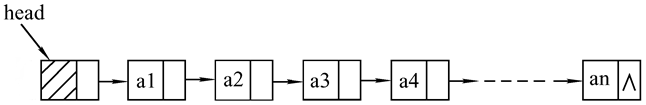
\includegraphics[width=3.36458in,height=0.55208in]{png-jpeg-pics/C20E94AE04F8208A15667A05019B1E65.png}

{b\textbf{. 双链表}\\
}

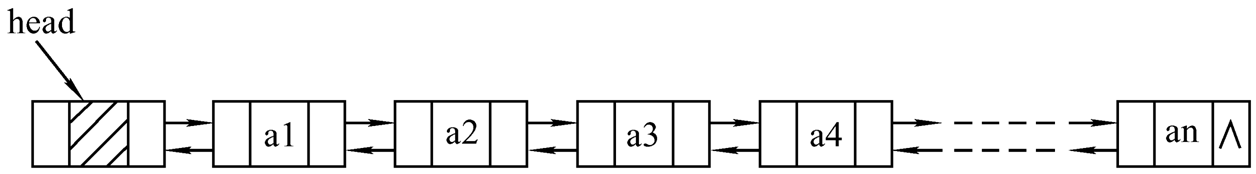
\includegraphics[width=3.33333in,height=0.45833in]{png-jpeg-pics/7D7C423781159DA1E482604156DD615A.png}

{c\textbf{. 循环单链表}\\
}

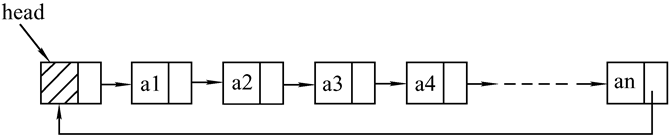
\includegraphics[width=3.48958in,height=0.71875in]{png-jpeg-pics/A73BFA643AA8FB8519FED189FD23A39C.png}

{d\textbf{. 循环双链表}\\
}

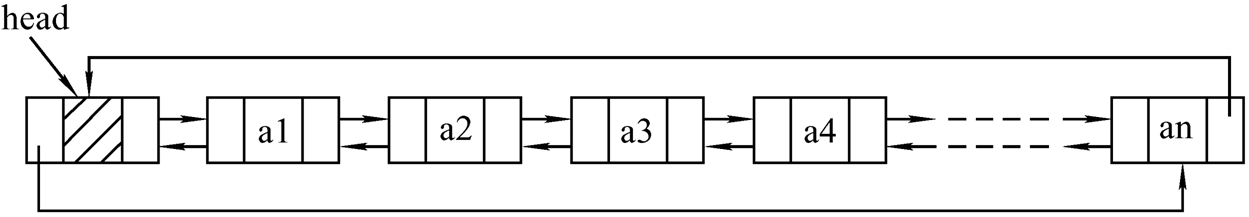
\includegraphics[width=3.33333in,height=0.58333in]{png-jpeg-pics/7E10782F7D3284B6634F5CB34D06A188.png}

{e\textbf{. 静态链表}\\
}

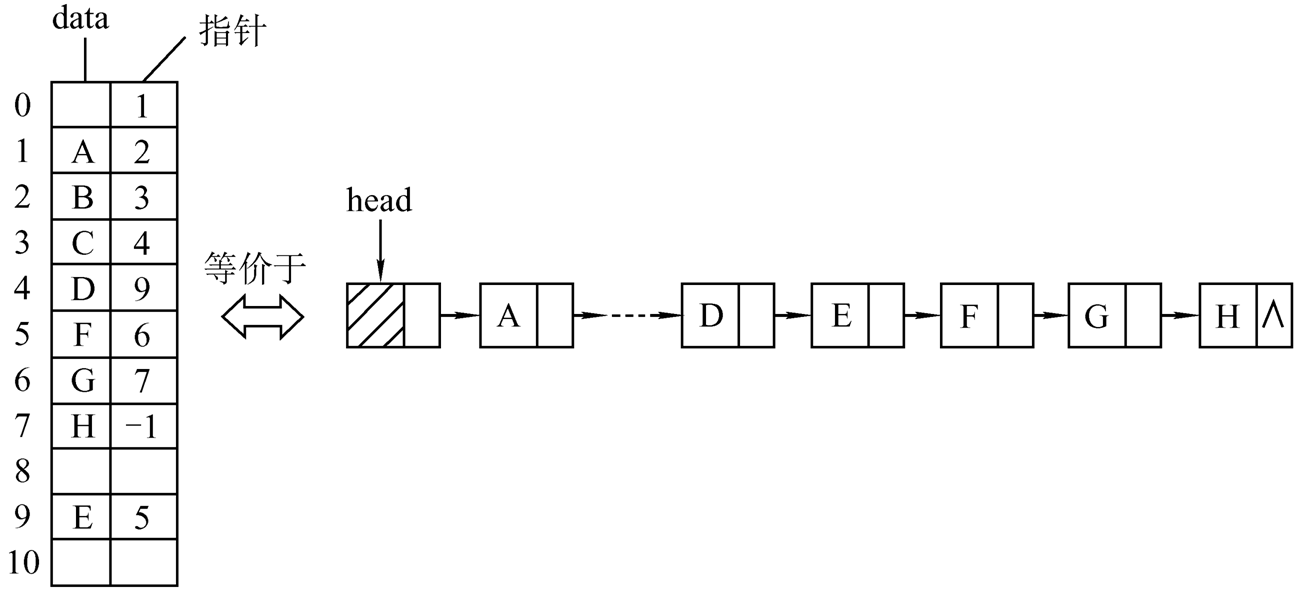
\includegraphics[width=3.33333in,height=1.51042in]{png-jpeg-pics/DBE33BB1E0A5E477AF148176D1253920.png}
